\section{Security and Availability}

\subsection{Failure controls and receiver validation}

The evaluation injects invalid signature, wrong receipt, expiry, replay, unknown peer, disallowed import type, monitor-only policy, receiver unavailability, authorization timeout, restart, stale decision, session termination, and late-context conditions. In every tested condition, the receiver either rejects the context or applies its own disposition. Appendix~\ref{app:extended-results} reports the full source-control matrix; Table~\ref{tab:protocol-assurance} adds the validation-value mutation corpus.

The controls establish the boundary conditions for the result. A malformed or stale context does not create a restriction in the exercised path. A correlated but late context can be retained without being counted as prevention. A timeout or receiver outage resolves through Domain B's policy.

\subsection{Valid hostile peers}

Signature validation authenticates the issuer; it does not establish that the issuer's observation is true. The hostile-peer study therefore sends syntactically valid warnings from an authorized peer at increasing synthetic burst sizes. At the \HostileBurstWarnings-warning burst, the current containment-first policy accepts and constrains \HostileCurrentConstrained{} warnings. Idempotence accepts and constrains \HostileIdempotentConstrained{} warning while deduplicating \HostileIdempotentDeduplicated{}. The quota-plus-monitor response constrains \HostileQuotaConstrained{} warnings and monitors \HostileQuotaMonitored{}.

This result makes the receiver's policy choice explicit. A broad arrival-triggered guard can be used to impose availability cost, even when the peer is syntactically valid. Idempotence reduces repeated collateral restriction for a single warning. Quota-plus-monitor provides a measured overload posture in the tested burst: a receiver limits automatic restriction and retains excess warnings for local monitoring. The sweep is synthetic and does not estimate an operational warning rate.

\subsection{Security-availability trade-off}

Containment-first has a material availability cost in the selected synthetic false-warning treatments. In the inside-window early and boundary treatments, \InsideWindowBenignConstrained{} of \InsideWindowBenignAttempted{} benign agent calls are constrained and \InsideWindowWorkflowCompleted{} of \InsideWindowWorkflowTotal{} affected workflows complete. The remaining no-evidence and late treatments forward \OutsideWindowBenignForwarded{} of \OutsideWindowBenignAttempted{} benign agent calls and complete \OutsideWindowWorkflowCompleted{} of \OutsideWindowWorkflowTotal{} workflows. The aggregate \WorkflowCompleted{} of \WorkflowTotal{} result is reported for accounting, but does not blend away the treatment-specific false-warning cost.

\begin{figure}[t]
\centering
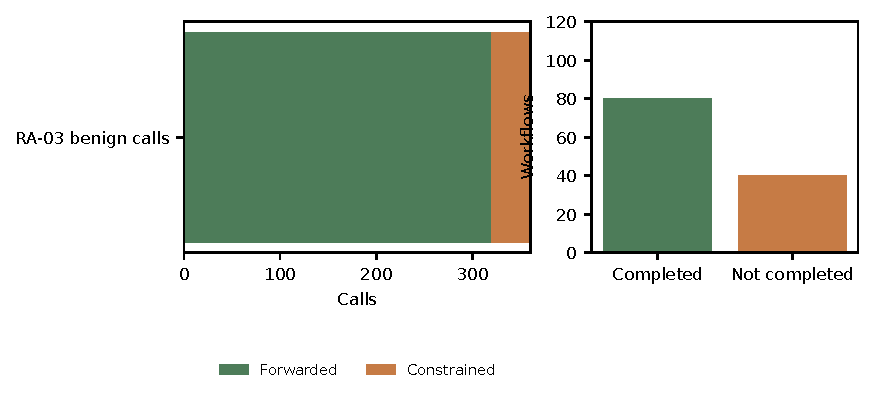
\includegraphics[width=\columnwidth]{security-availability}
\caption{Measured availability cost in the selected RA-03 synthetic workload.}
\label{fig:availability}
\end{figure}

\begin{table*}[t]\centering\scriptsize
\caption{Measured RA-03 availability cost under selected synthetic false-warning treatments and capability restriction; this is not a universal false-positive rate.}
\begin{tabular}{@{}p{0.22\textwidth}rrrp{0.23\textwidth}p{0.21\textwidth}@{}}\toprule
Treatment group & Attempted & Forwarded & Constrained & Workflow completion & Affected capability \\ \midrule
Inside-window early and boundary & \InsideWindowBenignAttempted & \InsideWindowBenignForwarded & \InsideWindowBenignConstrained & \InsideWindowWorkflowCompleted/\InsideWindowWorkflowTotal & repository.write in frozen benign metadata workflow \\
No context, outside window, post-detection, and post-containment & \OutsideWindowBenignAttempted & \OutsideWindowBenignForwarded & 0 & \OutsideWindowWorkflowCompleted/\OutsideWindowWorkflowTotal & no restriction in these treatments \\ \midrule
All selected treatments & \BenignAttempted & \BenignForwarded & \BenignConstrained & \WorkflowCompleted/\WorkflowTotal (\WorkflowCompletionRate) & selected synthetic capability restriction \\ \bottomrule
\end{tabular}\label{tab:utility}\end{table*}


The reported cohort establishes a bounded receiver-strategy frontier. Never restricting forwards the selected benign workload. Standing Guard maximizes blocking but constrains the capability continuously. Arrival Guard activates the same class-wide guard after accepted context becomes actionable. Exact Binding preserves containment on the accepted exact-binding subset while narrowing the restriction to that binding. The post-denial substitution and frontier studies add Campaign Correlation, which covers the declared related substitutions that Exact Binding alone permits.

\subsection{External-warning coverage and admission}

A credential-free successor evaluates the complete sealed external ledger from the pinned AgentDojo commit \cite{agentDojo} and pinned Prompt Guard 2 86M output configuration \cite{promptGuardTwo}; it consumes preserved detector outputs rather than rerunning the detector. Its declared normalizer maps \texttt{LABEL\_0} to no warning and \texttt{LABEL\_1} to a TCX prompt-attack category. Table~\ref{tab:independent-warning-full-pipeline} separates source coverage, detector output, normalization, receiver admission, and exact binding. Of \ExternalWarningFullAttackCases{} attack-bearing source cases, \ExternalWarningFullWarnings{} produce a warning and an admitted exact binding; \ExternalWarningFullAttackNoWarning{} produce no warning and therefore no actionable TCOP evidence. TCOP cannot compensate for a detector no-warning result.

Table~\ref{tab:independent-warning-full-outcomes} reports every policy over all \ExternalWarningFullSourceCases{} external source cases. Arrival Guard, Exact Binding, and Campaign Correlation block \ExternalWarningFullCTwoBlocked{} of \ExternalWarningFullAttackCases{} harmful actions, the \ExternalWarningFullConditionalNumerator{} for which accepted exact evidence exists, and forward the remaining \ExternalWarningFullCTwoForwarded{} no-warning harmful actions. They forward all \ExternalWarningFullBenignCases{} benign no-warning actions. Standing Guard blocks \ExternalWarningFullCThreeBlocked{} of \ExternalWarningFullAttackCases{} harmful actions but constrains all \ExternalWarningFullCThreeBenignConstrained{} of \ExternalWarningFullBenignCases{} benign actions because it is a standing receiver guard. This is an integration and authorization-coverage result, not an estimate of detector quality, warning prevalence, or deployment effectiveness.

Table~\ref{tab:independent-warning-v2-controls} adds deliberately derived protocol controls to the selected external bases. Exact Binding and Campaign Correlation apply no restriction to partial or mismatched bindings. Stale and replayed context are rejected before policy. Sender-suggested-only relation information remains nonrestrictive under Campaign Correlation. Campaign Correlation forwards all \ExternalWarningVTwoNoRelationCTwoEForwarded{} harmful substitutions without a receiver-created relation, including \ExternalWarningVTwoSessionNoRelationForwarded{} session-lineage and \ExternalWarningVTwoDelegationNoRelationForwarded{} delegation variants; it blocks all \ExternalWarningVTwoWithRelationCTwoEBlocked{} paired substitutions when the receiver has created the corresponding local relation. These controls demonstrate the declared receiver logic, not a general claim about correlation quality.

\begin{table}[t]\centering\scriptsize
\caption{Full external-warning pipeline coverage. All \ExternalWarningFullSourceCases{} cases in the sealed detector-output ledger are evaluated; a warning is not a detector-quality estimate.}
\begin{tabular}{@{}p{0.62\columnwidth}r@{}}\toprule
Stage or source category & Cases \\ \midrule
Attack-bearing source cases & \ExternalWarningFullAttackCases \\
\quad Detector warning $\rightarrow$ normalized TCX $\rightarrow$ admitted exact binding & \ExternalWarningFullWarnings/\ExternalWarningFullNormalized/\ExternalWarningFullAdmitted \\
\quad Detector no-warning $\rightarrow$ no actionable TCOP evidence & \ExternalWarningFullAttackNoWarning \\
Benign source cases, all detector no-warning & \ExternalWarningFullBenignCases \\
Total no actionable evidence & \ExternalWarningFullNoActionable \\ \bottomrule
\end{tabular}\label{tab:independent-warning-full-pipeline}\end{table}

\begin{table*}[t]\centering\scriptsize
\caption{Full-population receiver authorization outcomes over \ExternalWarningFullAttackCases{} attack-bearing and \ExternalWarningFullBenignCases{} benign external source cases. Arrival Guard, Exact Binding, and Campaign Correlation use accepted evidence conditionally; Standing Guard is a standing local restriction.}
\begin{tabular}{@{}lrr|rr@{}}\toprule
Policy & \shortstack{Harmful\\blocked} & \shortstack{Harmful\\forwarded} & \shortstack{Benign\\constrained} & \shortstack{Benign\\forwarded} \\ \midrule
Local Only (C0) & \ExternalWarningFullCZeroBlocked/\ExternalWarningFullAttackCases & \ExternalWarningFullCZeroForwarded/\ExternalWarningFullAttackCases & \ExternalWarningFullCZeroBenignConstrained/\ExternalWarningFullBenignCases & \ExternalWarningFullCZeroBenignForwarded/\ExternalWarningFullBenignCases \\
Arrival Guard (C1) & \ExternalWarningFullCOneBlocked/\ExternalWarningFullAttackCases & \ExternalWarningFullCOneForwarded/\ExternalWarningFullAttackCases & \ExternalWarningFullCOneBenignConstrained/\ExternalWarningFullBenignCases & \ExternalWarningFullCOneBenignForwarded/\ExternalWarningFullBenignCases \\
Exact Binding (C2) & \ExternalWarningFullCTwoBlocked/\ExternalWarningFullAttackCases & \ExternalWarningFullCTwoForwarded/\ExternalWarningFullAttackCases & \ExternalWarningFullCTwoBenignConstrained/\ExternalWarningFullBenignCases & \ExternalWarningFullCTwoBenignForwarded/\ExternalWarningFullBenignCases \\
Campaign Correlation (C2E) & \ExternalWarningFullCTwoEBlocked/\ExternalWarningFullAttackCases & \ExternalWarningFullCTwoEForwarded/\ExternalWarningFullAttackCases & \ExternalWarningFullCTwoEBenignConstrained/\ExternalWarningFullBenignCases & \ExternalWarningFullCTwoEBenignForwarded/\ExternalWarningFullBenignCases \\
Standing Guard (C3) & \ExternalWarningFullCThreeBlocked/\ExternalWarningFullAttackCases & \ExternalWarningFullCThreeForwarded/\ExternalWarningFullAttackCases & \ExternalWarningFullCThreeBenignConstrained/\ExternalWarningFullBenignCases & \ExternalWarningFullCThreeBenignForwarded/\ExternalWarningFullBenignCases \\ \bottomrule
\end{tabular}\label{tab:independent-warning-full-outcomes}\end{table*}

\begin{table}[t]\centering\scriptsize
\caption{Independent Warning Admission v2 derived controls. Each row contains \ExternalWarningVTwoSelectedPositive{} derived cases. The substitution rows contain \ExternalWarningVTwoSessionNoRelationForwarded{} session-lineage and \ExternalWarningVTwoDelegationNoRelationForwarded{} delegation variants.}
\begin{tabular}{@{}p{0.51\columnwidth}p{0.38\columnwidth}@{}}\toprule
Control & Receiver result \\ \midrule
Partial binding & Exact Binding/Campaign Correlation: \ExternalWarningVTwoPartialCTwoERestricted/\ExternalWarningVTwoSelectedPositive{} restrictions \\
Mismatched binding & Exact Binding/Campaign Correlation: \ExternalWarningVTwoMismatchCTwoERestricted/\ExternalWarningVTwoSelectedPositive{} restrictions \\
Stale or replayed context & Campaign Correlation: \ExternalWarningVTwoStaleCTwoERejected/\ExternalWarningVTwoSelectedPositive{} rejected before policy \\
Sender-suggested-only relation & Campaign Correlation: \ExternalWarningVTwoSenderSuggestedCTwoERestricted/\ExternalWarningVTwoSelectedPositive{} restrictions \\
Harmful substitution, no B-local relation & Campaign Correlation: \ExternalWarningVTwoNoRelationCTwoEForwarded/\ExternalWarningVTwoSelectedPositive{} forwarded \\
Harmful substitution, B-local relation & Campaign Correlation: \ExternalWarningVTwoWithRelationCTwoEBlocked/\ExternalWarningVTwoSelectedPositive{} blocked \\ \bottomrule
\end{tabular}\label{tab:independent-warning-v2-controls}\end{table}


\subsection{Local overhead}

The performance experiment reports authorization, gateway, and warning-to-enforcement measurements separately for cache-disabled and fixed-time-to-live cache selections. The correctness and causal replays use the cache-disabled configuration. The local-harness measurements appear in Appendix~\ref{app:extended-results}.
